% Created 2025-01-21 Tue 12:28
% Intended LaTeX compiler: lualatex
\documentclass[bigger]{beamer}
\usepackage{amsmath}
\usepackage{fontspec}
\usepackage{graphicx}
\usepackage{longtable}
\usepackage{wrapfig}
\usepackage{rotating}
\usepackage[normalem]{ulem}
\usepackage{capt-of}
\usepackage{hyperref}
\usetheme[progressbar=foot, sectionpage=none, numbering=fraction]{metropolis}
\usepackage{tikz}
\usepackage{booktabs}
\usepackage{adjustbox}
\usepackage{diagbox}
\usepackage{latexcolors}
\usetikzlibrary{automata, positioning, arrows, arrows.meta}
\usepackage{diagbox}
\usepackage{dsfont}
\usepackage{amsmath}
\usepackage{fontawesome}
\usepackage{pgfgantt}
\usepackage[ruled]{algorithm2e}
\usepackage[absolute, overlay]{textpos}
\usepackage{xcolor}
\definecolor{UmlBlue}{HTML}{0067b1} \setbeamercolor{progress bar}{fg=UmlBlue} \setbeamercolor{title separator}{fg=UmlBlue}
\setbeamercolor{progress bar in head/foot}{fg=UmlBlue} \setbeamercolor{progress bar in section page}{fg=UmlBlue} \setbeamercolor{alerted text}{fg=UmlBlue}
\pretocmd{\tableofcontents}{\thispagestyle{empty}}{}{}
\usetheme{default}
\author{Andrea Pierré}
\date{January 21, 2025}
\title{DRL project update}
\subtitle{Cartesian/polar duplicated coordinates experiment}
\setbeamercovered{transparent=10}
\setbeamertemplate{section in toc}[sections numbered]
\AtBeginSection[]{\begin{frame}[plain, noframenumbering]{Outline}    \setbeamertemplate{section in toc}[sections numbered]\setbeamertemplate{subsection in toc}[subsections numbered]\tableofcontents[currentsection, currentsubsection]\end{frame}}
\AtBeginSubsection[]{\begin{frame}[plain, noframenumbering]{Outline}\setbeamertemplate{section in toc}[sections numbered]\setbeamertemplate{subsection in toc}[subsections numbered]\tableofcontents[currentsection,currentsubsection]\end{frame}}
\definecolor{headercolor}{HTML}{232323}
\setbeamercolor{normal text}{%
% bg=,
fg=headercolor
}
\hypersetup{
 pdfauthor={Andrea Pierré},
 pdftitle={DRL project update},
 pdfkeywords={},
 pdfsubject={},
 pdfcreator={Emacs 29.4 (Org mode 9.7.19)}, 
 pdflang={English}}
\begin{document}

\maketitle
\begin{frame}[plain]{Outline}
\tableofcontents
\end{frame}

\section{Current status}
\label{sec:org278a306}
\begin{frame}[label={sec:orgafd0086}]{Current status}
\begin{center}
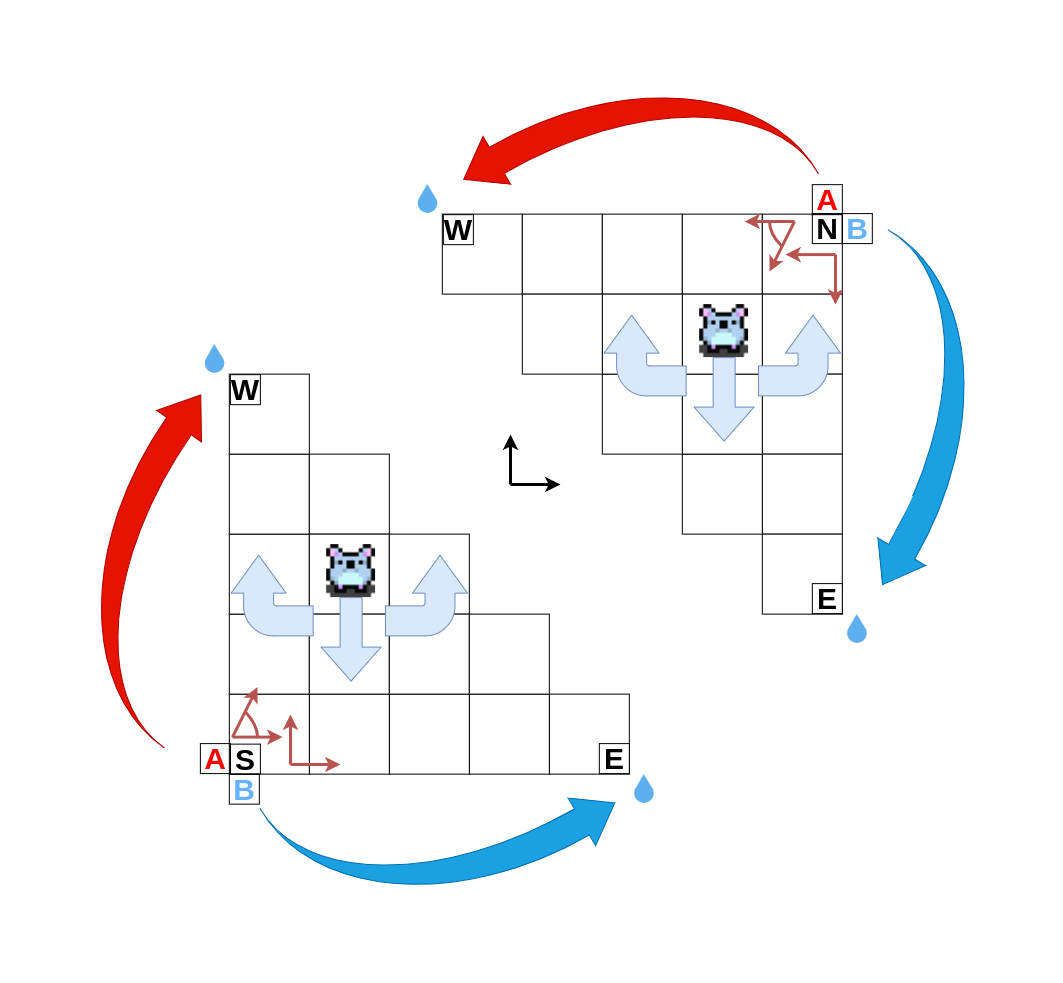
\includegraphics[height=0.6\textheight]{img/RL_env-cartesian-polar.drawio.png}
\end{center}
\begin{itemize}
\item Environment rewrite: done
\item Training: \textasciitilde{}4.5 hours to train 30 agents on both tasks on Oscar
\item Analysis: WIP
\end{itemize}
\end{frame}
\begin{frame}[label={sec:orgbaa7ef4}]{State space \& network architecture}
\begin{center}
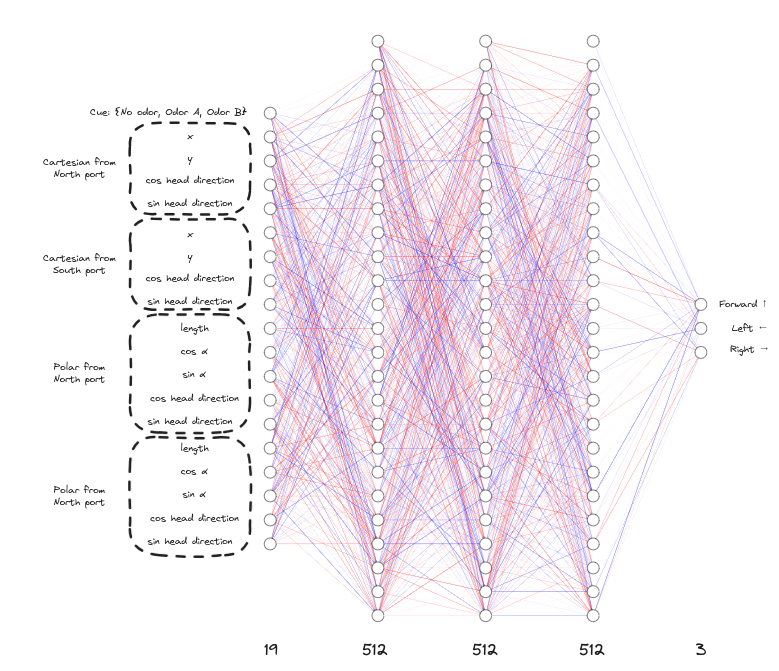
\includegraphics[height=0.95\textheight]{img/state-space-nn.png}
\end{center}
\end{frame}
\begin{frame}[label={sec:orgf41095c}]{Training}
East/West
\begin{center}
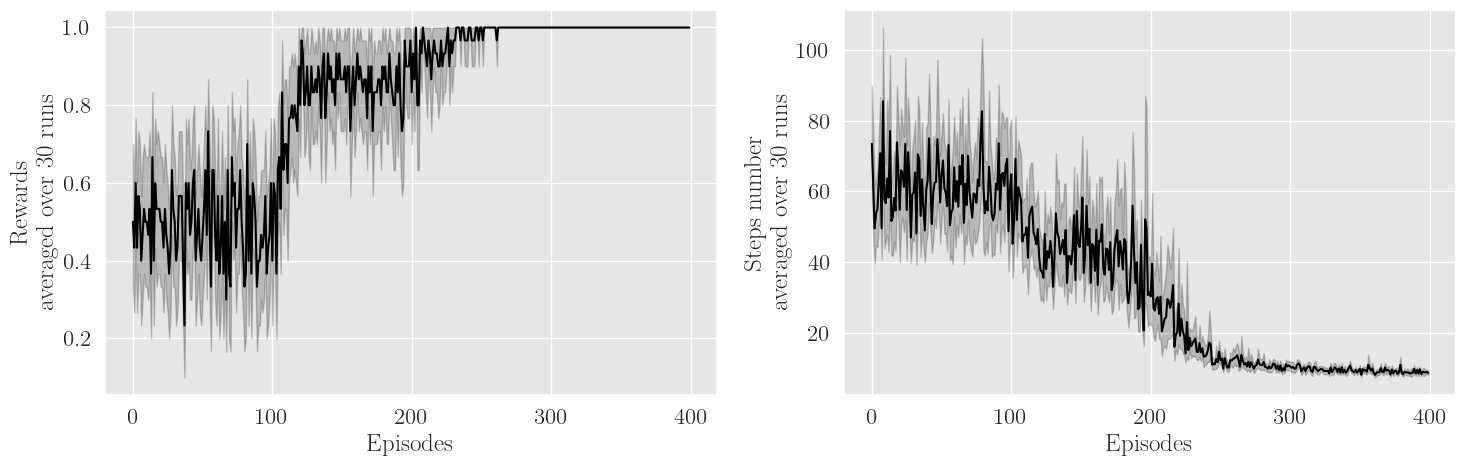
\includegraphics[height=0.35\textheight]{img/steps-and-rewards-EastWest.png}
\end{center}
Left/Right
\begin{center}
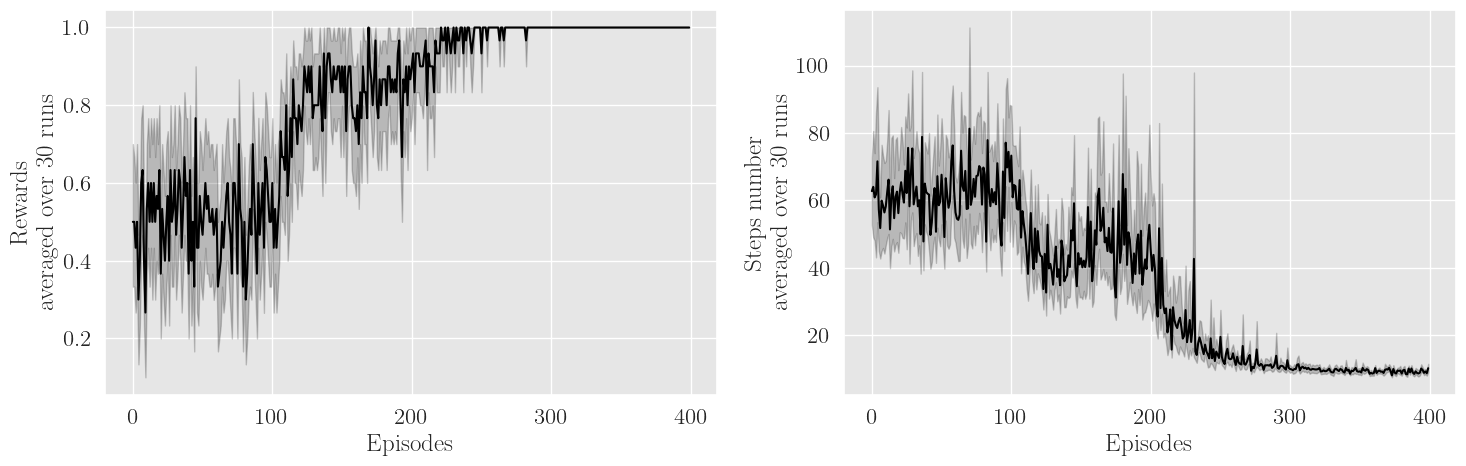
\includegraphics[height=0.35\textheight]{img/steps-and-rewards-LeftRight.png}
\end{center}
\end{frame}
\begin{frame}[label={sec:orga5fd31a}]{Training checks - East/West}
\begin{center}
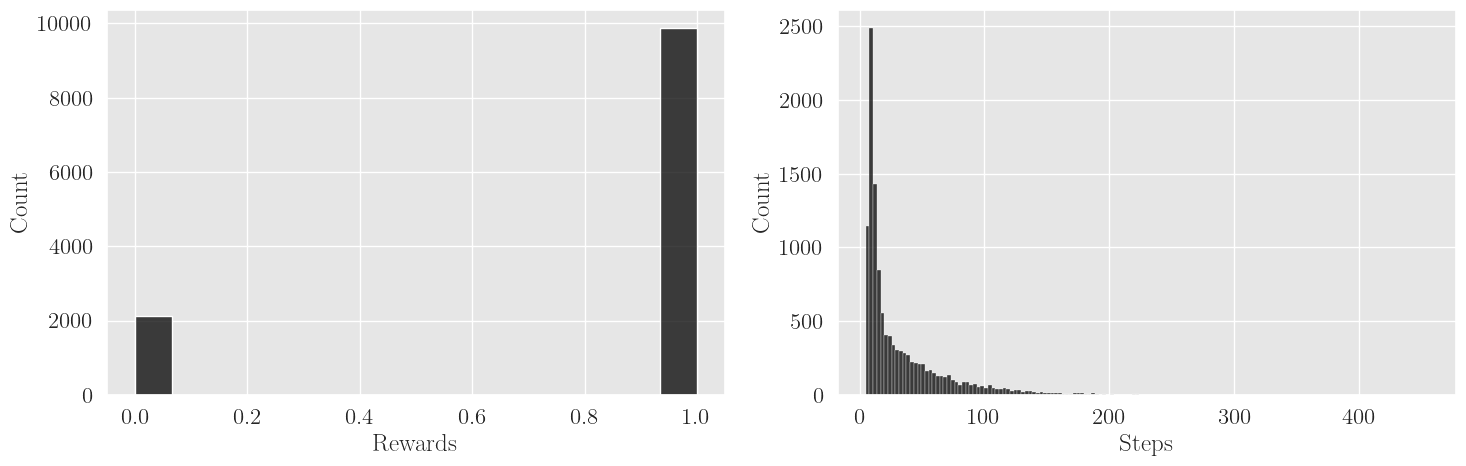
\includegraphics[width=\textwidth]{img/steps-and-rewards-distrib-EastWest.png}
\end{center}
\begin{columns}
\begin{column}[c]{0.5\columnwidth}
\begin{center}
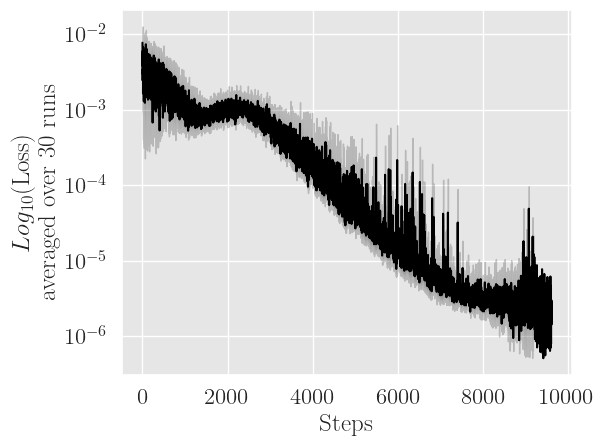
\includegraphics[width=0.8\textwidth]{img/loss-EastWest.png}
\end{center}
\end{column}
\begin{column}[c]{0.5\columnwidth}
\begin{center}
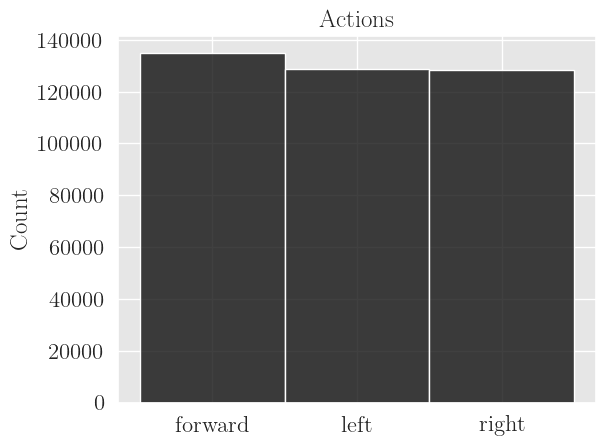
\includegraphics[width=0.65\textwidth]{img/actions-distribution-EastWest.png}
\end{center}
\end{column}
\end{columns}
\end{frame}
\begin{frame}[label={sec:org82d34ea}]{Training checks - Left/Right}
\begin{center}
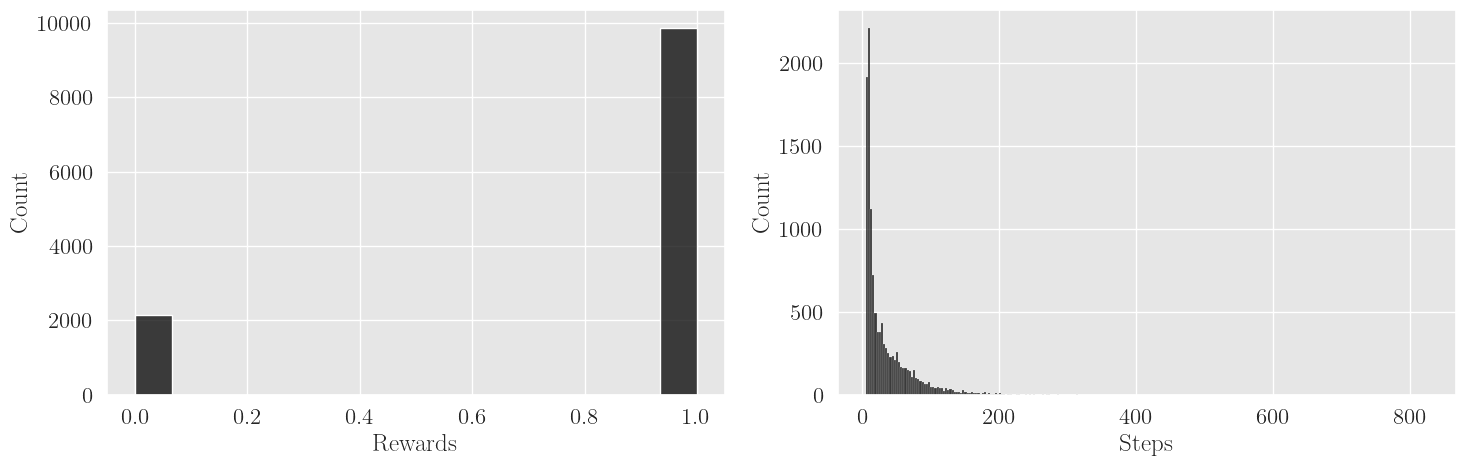
\includegraphics[width=\textwidth]{img/steps-and-rewards-distrib-LeftRight.png}
\end{center}
\begin{columns}
\begin{column}[c]{0.5\columnwidth}
\begin{center}
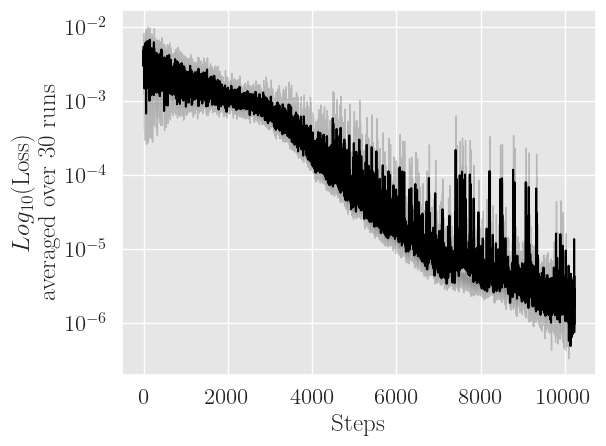
\includegraphics[width=0.8\textwidth]{img/loss-LeftRight.png}
\end{center}
\end{column}
\begin{column}[c]{0.5\columnwidth}
\begin{center}
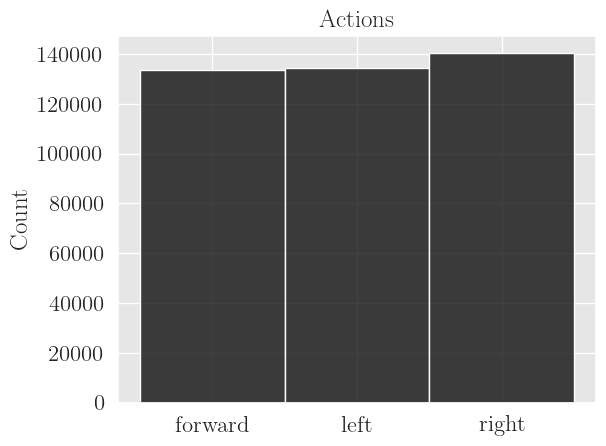
\includegraphics[width=0.65\textwidth]{img/actions-distribution-LeftRight.png}
\end{center}
\end{column}
\end{columns}
\end{frame}
\begin{frame}[label={sec:org3d777c1}]{Agent behavior}
\begin{columns}
\begin{column}[c]{0.3\columnwidth}
\begin{center}
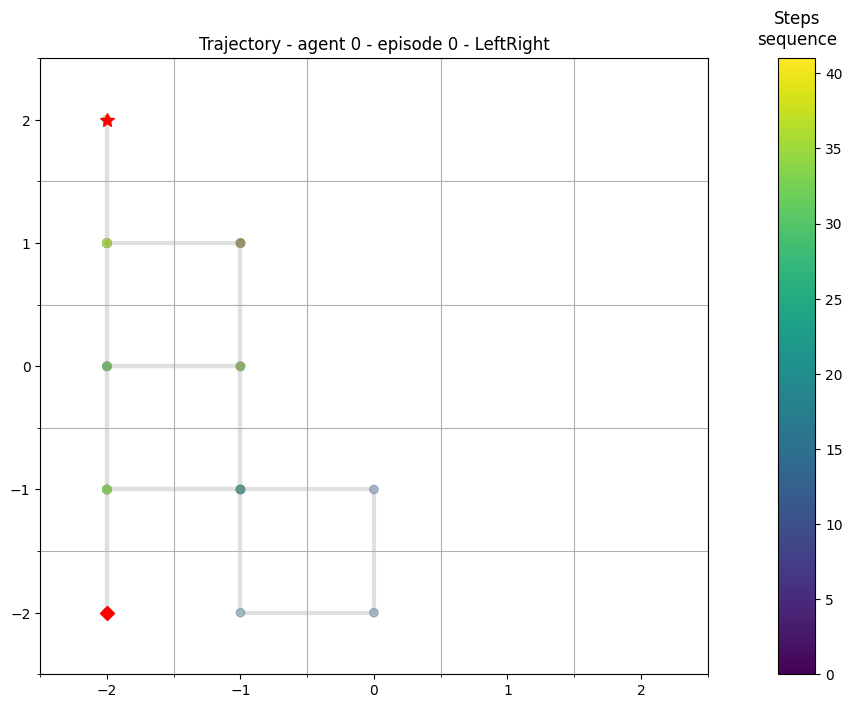
\includegraphics[height=0.28\textheight]{img/trajectory-0-0-LeftRight.png}
\end{center}
\begin{center}
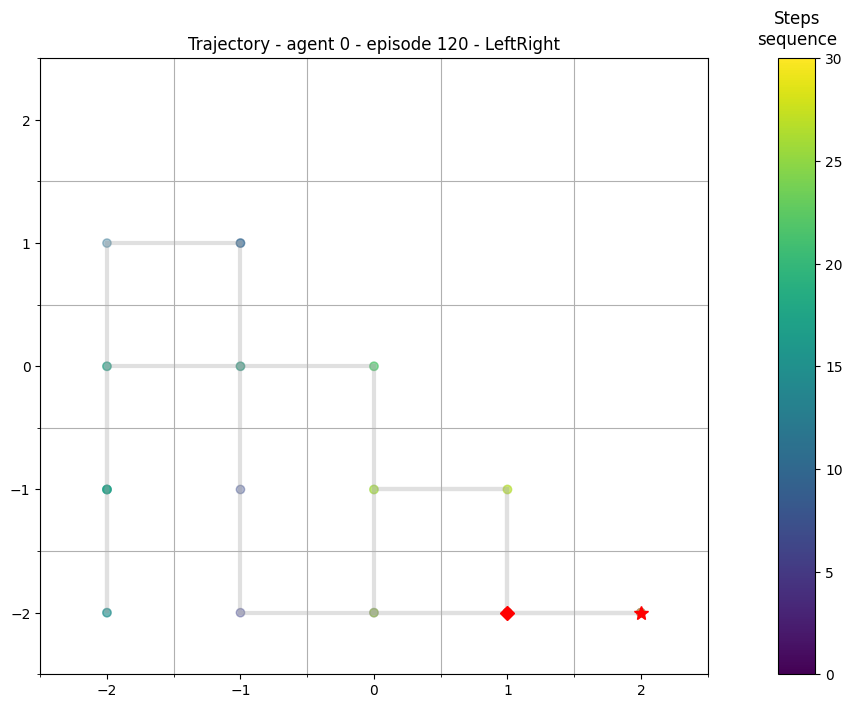
\includegraphics[height=0.28\textheight]{img/trajectory-0-120-LeftRight.png}
\end{center}
\begin{center}
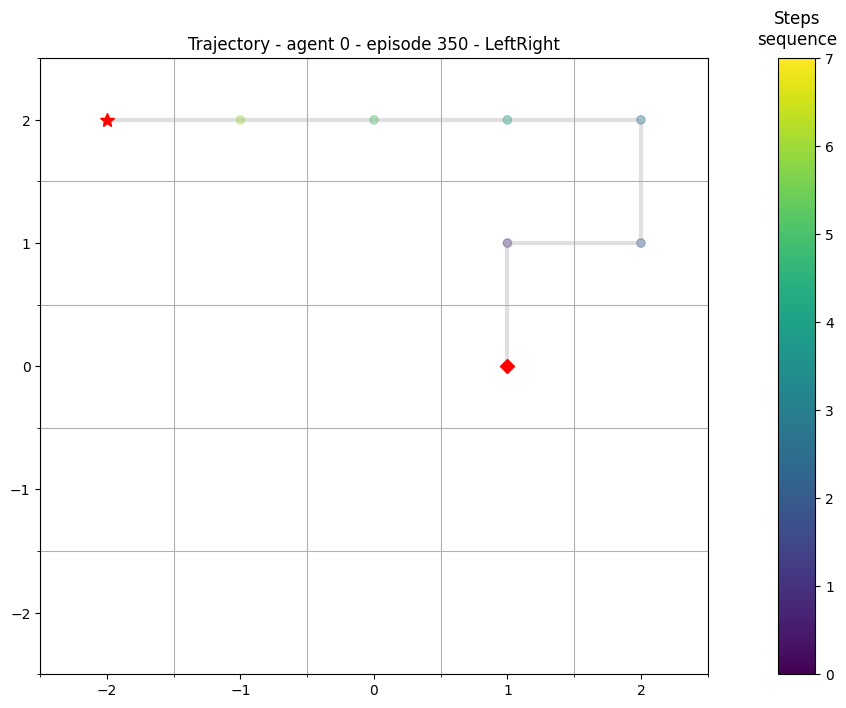
\includegraphics[height=0.28\textheight]{img/trajectory-0-350-LeftRight.png}
\end{center}
\end{column}
\begin{column}[c]{0.3\columnwidth}
\begin{center}
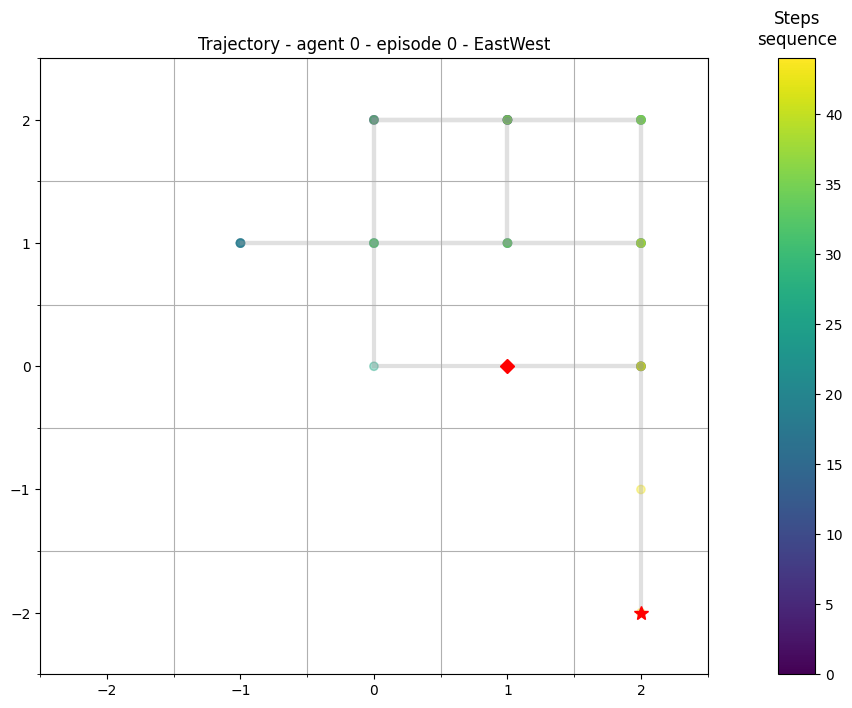
\includegraphics[height=0.28\textheight]{img/trajectory-0-0-EastWest.png}
\end{center}
\begin{center}
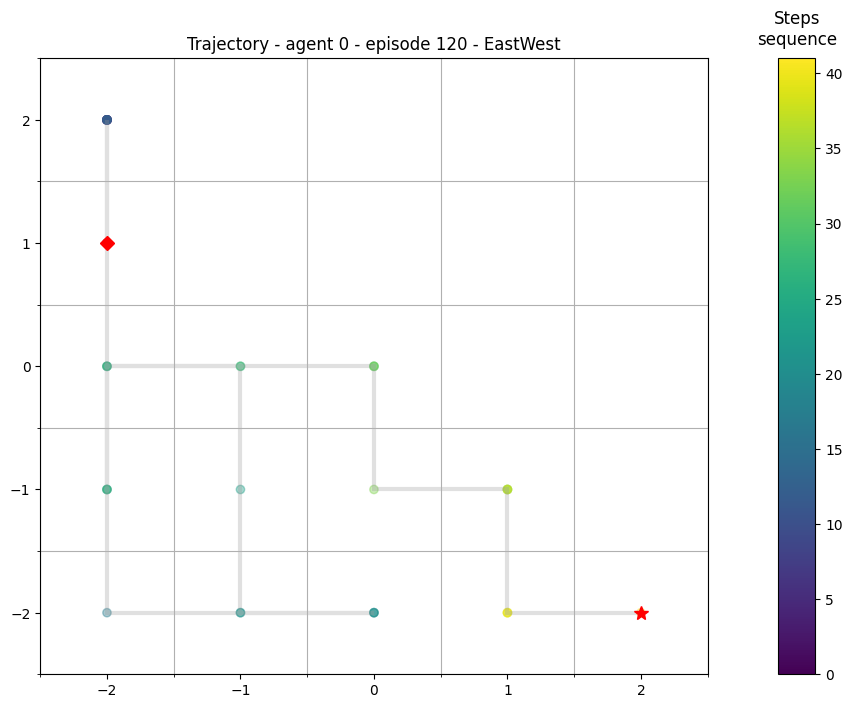
\includegraphics[height=0.28\textheight]{img/trajectory-0-120-EastWest.png}
\end{center}
\begin{center}
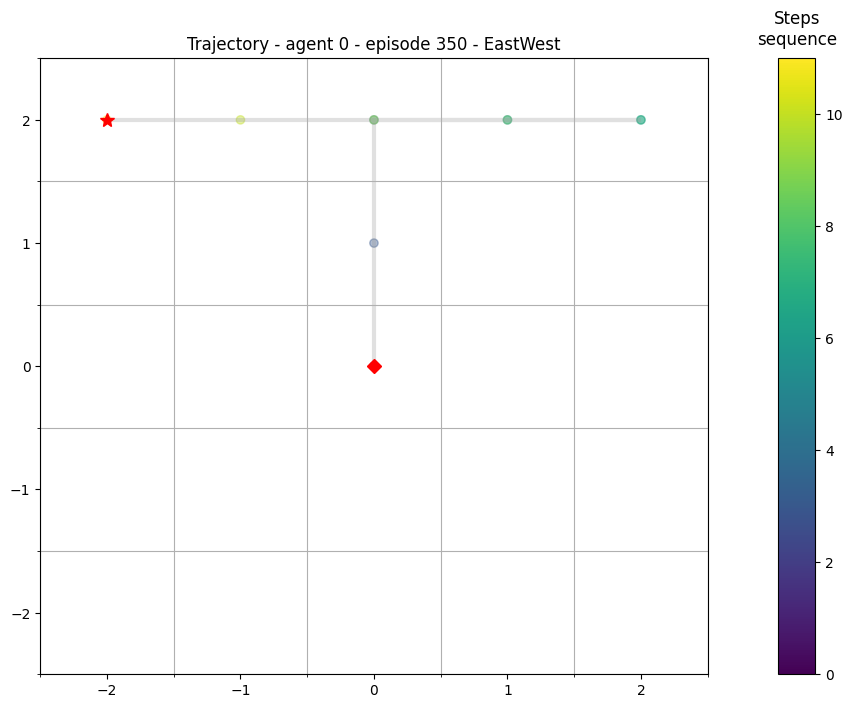
\includegraphics[height=0.28\textheight]{img/trajectory-0-350-EastWest.png}
\end{center}
\end{column}
\begin{column}[c]{0.25\columnwidth}
\begin{center}
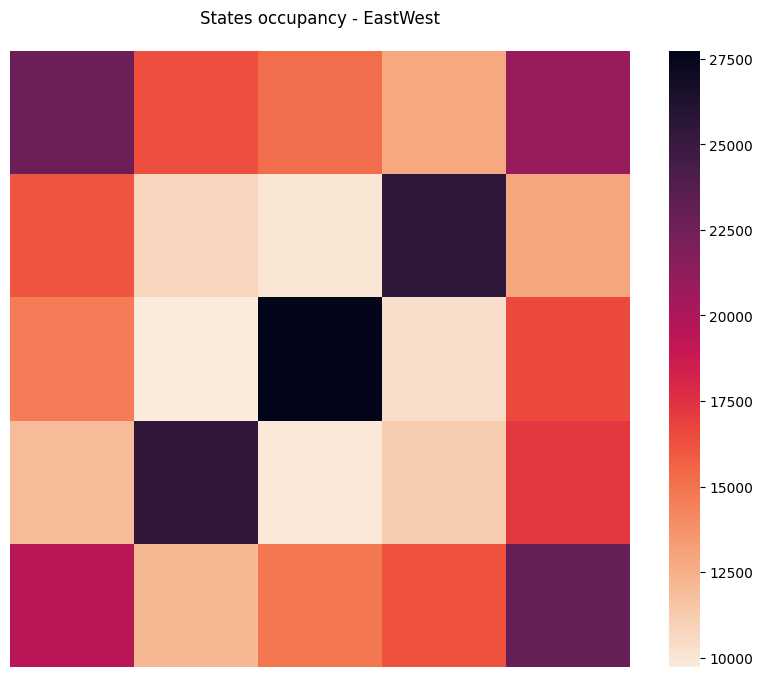
\includegraphics[width=\linewidth]{img/states-occupancy-EastWest.png}
\end{center}
\begin{center}
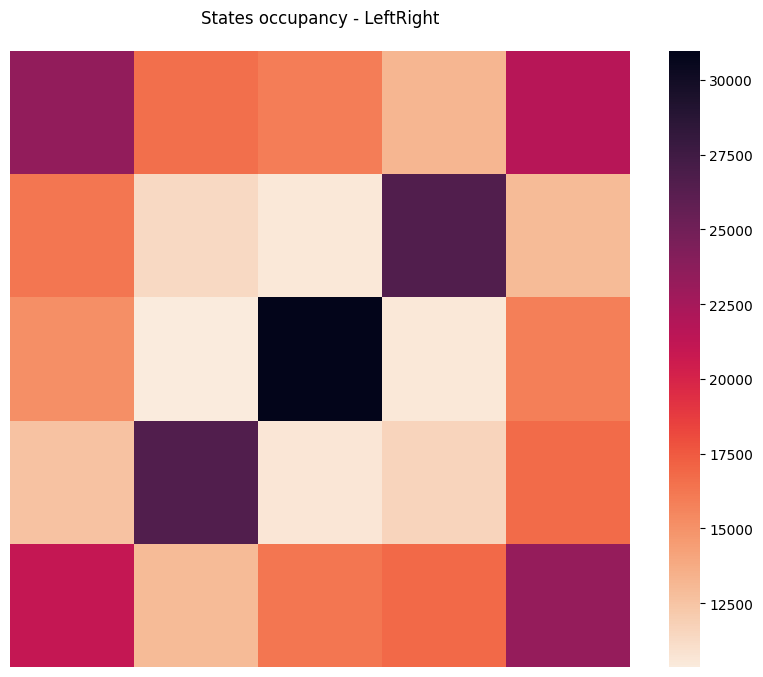
\includegraphics[width=\linewidth]{img/states-occupancy-LefRight.png}
\end{center}
\end{column}
\end{columns}
\end{frame}
\section{How to get insights at what the network learn?}
\label{sec:orge184218}
\begin{frame}[label={sec:org0c72e93}]{Activations learned - East/West}
\begin{center}
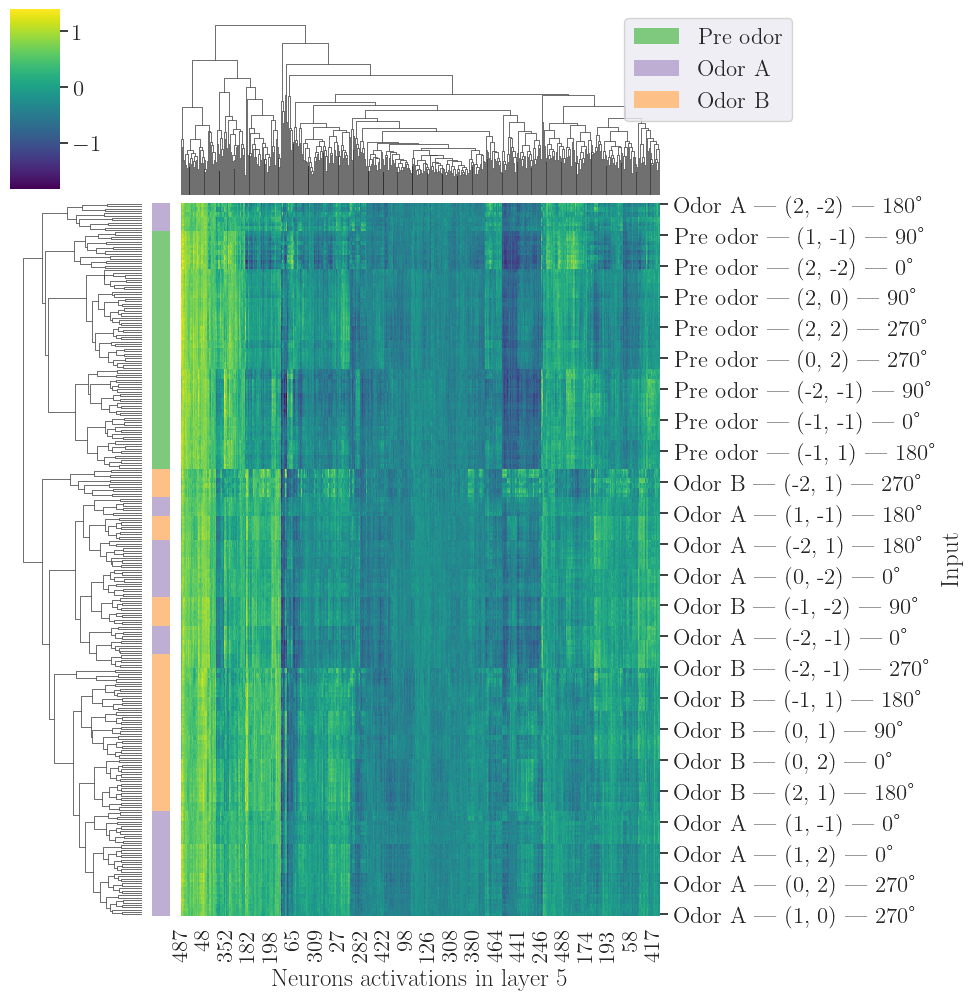
\includegraphics[height=0.9\textheight]{img/activations-learned-EastWest.png}
\end{center}
\end{frame}
\begin{frame}[label={sec:org3530d2a}]{Activations learned - Left/Right}
\begin{center}
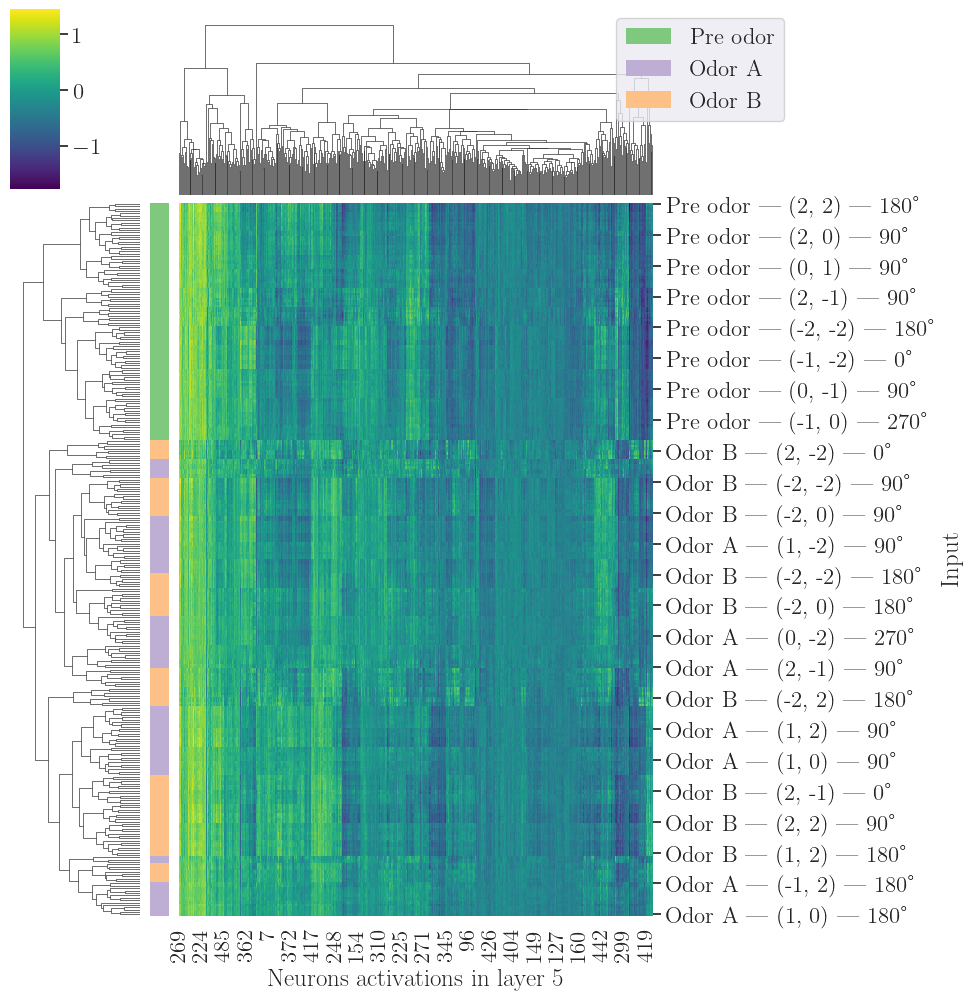
\includegraphics[height=0.9\textheight]{img/activations-learned-LeftRight.png}
\end{center}
\end{frame}
\begin{frame}[<+->][label={sec:orged4b1fd}]{Use the behavior as proxy}
\begin{itemize}
\item Silence the Cartesian/polar part of the input on a trained agent and look at how the agent behaves (x4 experiments)
\item Expectation:
\begin{itemize}
\item Left/right task:
\begin{itemize}
\item With the Cartesian inputs silenced \(\to\) the agent can solve the task
\item With the polar inputs silenced \(\to\) the agent struggle to solve the task
\end{itemize}
\item East/west task:
\begin{itemize}
\item With the Cartesian inputs silenced \(\to\) the agent can solve the task
\item With the polar inputs silenced \(\to\) the agent struggle to solve the task
\end{itemize}
\end{itemize}
\item Any other approach we could use?
\end{itemize}
\end{frame}
\begin{frame}[label={sec:org75b43c3}]{Neural representations?}
\begin{center}
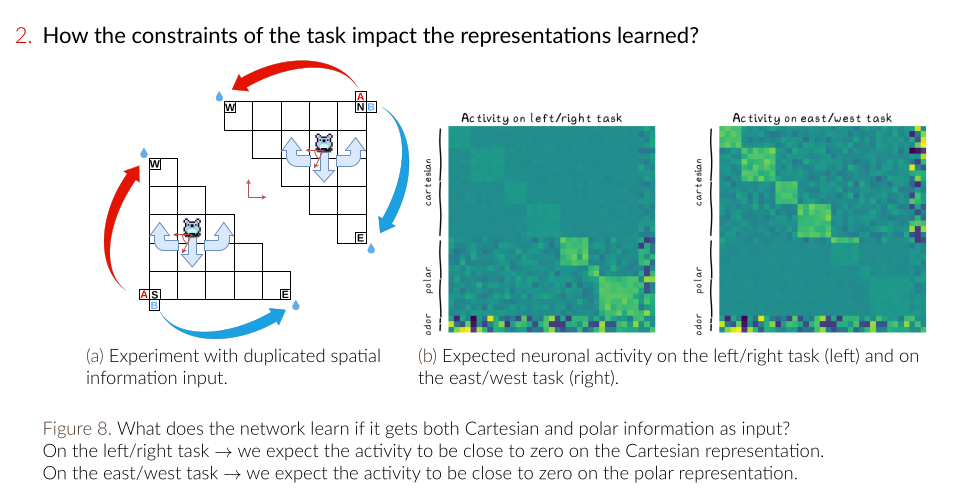
\includegraphics[width=.9\linewidth]{/home/kir0ul/Projects/RL_Olfaction/docs/expected cart-polar activations on both tasks.png}
\end{center}
\begin{itemize}
\item Need for some causal framework?
\end{itemize}
\end{frame}
\end{document}
